\begin{picture}(0,0)%
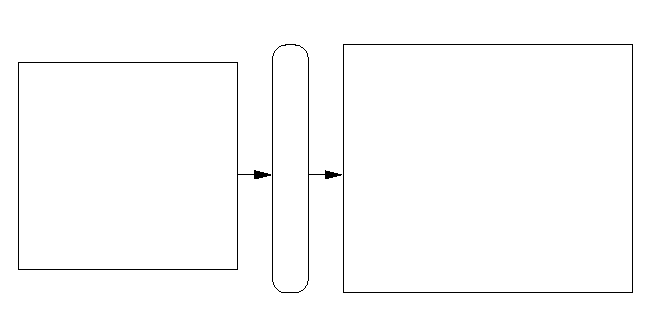
\includegraphics{img/tex/compiler}%
\end{picture}%
\setlength{\unitlength}{4144sp}%
%
\begingroup\makeatletter\ifx\SetFigFont\undefined%
\gdef\SetFigFont#1#2#3#4#5{%
  \reset@font\fontsize{#1}{#2pt}%
  \fontfamily{#3}\fontseries{#4}\fontshape{#5}%
  \selectfont}%
\fi\endgroup%
\begin{picture}(4704,2112)(-11,-1513)
\put(2566,209){\makebox(0,0)[lb]{\smash{\SetFigFont{10}{12.0}{\ttdefault}{\mddefault}{\updefault}{\color[rgb]{0,0,0}.globl main}%
}}}
\put(2566, 29){\makebox(0,0)[lb]{\smash{\SetFigFont{10}{12.0}{\ttdefault}{\mddefault}{\updefault}{\color[rgb]{0,0,0}~~~~.type main, @function}%
}}}
\put(2566,-121){\makebox(0,0)[lb]{\smash{\SetFigFont{10}{12.0}{\ttdefault}{\mddefault}{\updefault}{\color[rgb]{0,0,0}main:}%
}}}
\put(2566,-286){\makebox(0,0)[lb]{\smash{\SetFigFont{10}{12.0}{\ttdefault}{\mddefault}{\updefault}{\color[rgb]{0,0,0}~~~~pushhl \%ebp}%
}}}
\put(2566,-451){\makebox(0,0)[lb]{\smash{\SetFigFont{10}{12.0}{\ttdefault}{\mddefault}{\updefault}{\color[rgb]{0,0,0}~~~~movl \%esp, \%ebp}%
}}}
\put(2566,-616){\makebox(0,0)[lb]{\smash{\SetFigFont{10}{12.0}{\ttdefault}{\mddefault}{\updefault}{\color[rgb]{0,0,0}~~~~pushl \$.LC0}%
}}}
\put(2566,-781){\makebox(0,0)[lb]{\smash{\SetFigFont{10}{12.0}{\ttdefault}{\mddefault}{\updefault}{\color[rgb]{0,0,0}~~~~call puts}%
}}}
\put(2566,-946){\makebox(0,0)[lb]{\smash{\SetFigFont{10}{12.0}{\ttdefault}{\mddefault}{\updefault}{\color[rgb]{0,0,0}~~~~addl \$4, \%esp}%
}}}
\put(2566,-1111){\makebox(0,0)[lb]{\smash{\SetFigFont{10}{12.0}{\ttdefault}{\mddefault}{\updefault}{\color[rgb]{0,0,0}.L1:}%
}}}
\put(2566,-1276){\makebox(0,0)[lb]{\smash{\SetFigFont{10}{12.0}{\ttdefault}{\mddefault}{\updefault}{\color[rgb]{0,0,0}~~~~leave}%
}}}
\put(2566,-1441){\makebox(0,0)[lb]{\smash{\SetFigFont{10}{12.0}{\ttdefault}{\mddefault}{\updefault}{\color[rgb]{0,0,0}~~~~ret}%
}}}
\put(2116,-916){\rotatebox{90.0}{\makebox(0,0)[lb]{\smash{\SetFigFont{10}{12.0}{\sfdefault}{\mddefault}{\updefault}{\color[rgb]{0,0,0}compiler}%
}}}}
\put(3331,479){\makebox(0,0)[lb]{\smash{\SetFigFont{10}{12.0}{\sfdefault}{\mddefault}{\updefault}{\color[rgb]{0,0,0}main.s}%
}}}
\put(136, 29){\makebox(0,0)[lb]{\smash{\SetFigFont{10}{12.0}{\ttdefault}{\mddefault}{\updefault}{\color[rgb]{0,0,0}int puts(char *s);}%
}}}
\put(136,-331){\makebox(0,0)[lb]{\smash{\SetFigFont{10}{12.0}{\ttdefault}{\mddefault}{\updefault}{\color[rgb]{0,0,0}extern int var\_{}a;}%
}}}
\put(136,-691){\makebox(0,0)[lb]{\smash{\SetFigFont{10}{12.0}{\ttdefault}{\mddefault}{\updefault}{\color[rgb]{0,0,0}main()}%
}}}
\put(136,-871){\makebox(0,0)[lb]{\smash{\SetFigFont{10}{12.0}{\ttdefault}{\mddefault}{\updefault}{\color[rgb]{0,0,0}\{}%
}}}
\put(136,-1051){\makebox(0,0)[lb]{\smash{\SetFigFont{10}{12.0}{\ttdefault}{\mddefault}{\updefault}{\color[rgb]{0,0,0}~~puts("hello");}%
}}}
\put(136,-1231){\makebox(0,0)[lb]{\smash{\SetFigFont{10}{12.0}{\ttdefault}{\mddefault}{\updefault}{\color[rgb]{0,0,0}\}}%
}}}
\put(586,344){\makebox(0,0)[lb]{\smash{\SetFigFont{10}{12.0}{\sfdefault}{\mddefault}{\updefault}{\color[rgb]{0,0,0}main.i}%
}}}
\end{picture}
